\subsection{Convolutional Neural Networks}
  Convolutional Neural networks(CNN) have been prominent in the field of Computer vision in recent years.
  CNNs have been used in field of computer vision in order to classify images with high accuracy and speed \cite{razavian2014}.
  CNNs come at the cost of requiring long times to train using GPUs \cite{krizhevsky2012}.
  This makes standard use of CNNs impractical for tracking unknown objects, training a CNN online results in impairment of the system's speed \cite{bertinetto2016}.

  \subsubsection{Multi-domain CNNs}
  \citeauthor{CNNTracking} \cite{CNNTracking} use a CNN as the basis of the trakcer that they implement.
  The CNN is trained on a large, labelled dataset of videos to obtain a generic target representation.
  Training is done on one separate domain at a time, all the domains are worked through in an iterative process.
  This provides a CNN that can distinguish between target and background for an object in any of the trained domains.

  \begin{figure}[!ht]
    \centering
    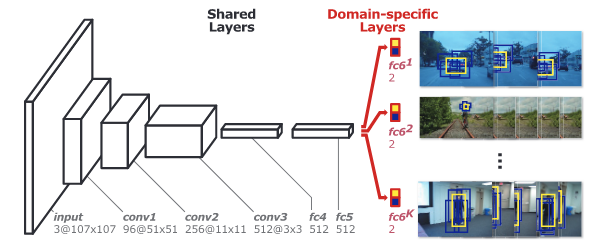
\includegraphics[scale=0.5]{MDNet.png}
    \label{fig:mdnet}
    \caption{The architecture of the Multi-Domain Network, from \cite{CNNTracking}}
  \end{figure}
  The output of this CNN is branched and given as input to domain-specific layers, see Figure~\ref{fig:mdnet}.
  The domain-specific layers are binary classifiers that can track the target object in a video stream.
  The domain-specific alyers are further trained online, using the video stream as input.

  \subsubsection{Convolutional Siamese Neural Networks}
  \citeauthor{bertinetto2016} \cite{bertinetto2016} offer a solution to the problem of tracking an unknown object with Convolutional Neural networks.
  The solution given by \citeauthor{bertinetto2016} is to train, offline, a CNN that solves the more general similarity problem.
  A function $f(z,x)$ is learned, the funtion compares images $x$ and $z$ and returns a value that estimates how similar the images are.
  A siamese neural network, two identical neural networks conjoined at the output node \cite{bromley1993}, is used to learn the similarity relation.

  A \textit{fully-convolutional}, translation invariant, siamese network is suggested by \citeauthor{bertinetto2016}.
  The fully-convolutional network allows for a whole frame to be searched in one pass of the image.
  This produces better results than sliding window techniques \cite{kang2014}.

  \subsubsection{Crowd Segmentation with CNNs}
  

